\documentclass[a4paper]{article}
\usepackage[letterpaper,margin=1in]{geometry}
\usepackage{blindtext}
\usepackage{lastpage}
\usepackage{fancyhdr}
\usepackage{setspace}
\usepackage{amsmath}
\usepackage{graphicx}
\usepackage{float}
\graphicspath{{./Figures}}

% Configure the header
\pagestyle{fancy} % Enable fancy headers
\fancyhead[L]{CE 591} % Left-aligned header
\fancyhead[C]{Wave Hydrodynamics} % Centered header
\fancyhead[R]{26/03/2025} % Right-aligned header

\onehalfspacing

\begin{document}

\begin{center}
\textbf{\large{Homework \#1}}

Bilge Kutay - 2511798
\end{center}

\textbf{Question 1:} Select a coastal engineering problem (in regional scale), and discuss which
governing equations can be used to model the waves for your selected problem. Explain the reason
why you have selected these equations with a few paragraphs.
\vspace{0.3cm}

A key problem in coastal engineering involves modeling non-linear wave transformation as waves propagate from deep to shallow water. This process includes shoaling, refraction, and breaking, which are governed by the Boussinesq equations and the Korteweg-de Vries (KdV) equation. These equations are selected for their ability to balance nonlinear and dispersive effects, critical for simulating wave behavior in shallow coastal zones.

The Boussinesq equations simplify the Navier-Stokes equations by retaining nonlinear and dispersive terms while reducing complexity. Unlike linear wave theory, which assumes small wave amplitudes and ignores non-linear interactions, the Boussinesq captures wave steepening, energy transfer, and frequency dispersion. This makes it effective for predicting wave asymmetry and breaking in shallow water.

The KdV equation supports this approach by focusing on weakly non-linear and weakly dispersive waves, such as solitary waves or long waves in shallow water. It provides a simplified model for unidirectional wave propagation, ideal for scenarios like tsunami evolution or wave deformation over gentle slopes. While higher-order Stokes theories are accurate for deep-water waves, they become impractical in shallow environments due to their reliance on perturbation methods.

In summary, the Boussinesq and KdV equations provide a practical mathematical foundation for modeling wave transformation, addressing the limitations of linear theory and higher-order Stokes models. 

\vspace{0.5cm}
\textbf{Question 2:} Considering Stokes’ second-order wave theory for monochromatic waves,
do the following computations and compare your results with the solutions from linear theory. Take
wave height H = 3 m, wave period T = 8 s and water depth h = 25 m.
\vspace{0.3cm}

\textbf{(a)} Plot the surface elevation for at least one wave period.
\begin{figure}[H]
    \centering
    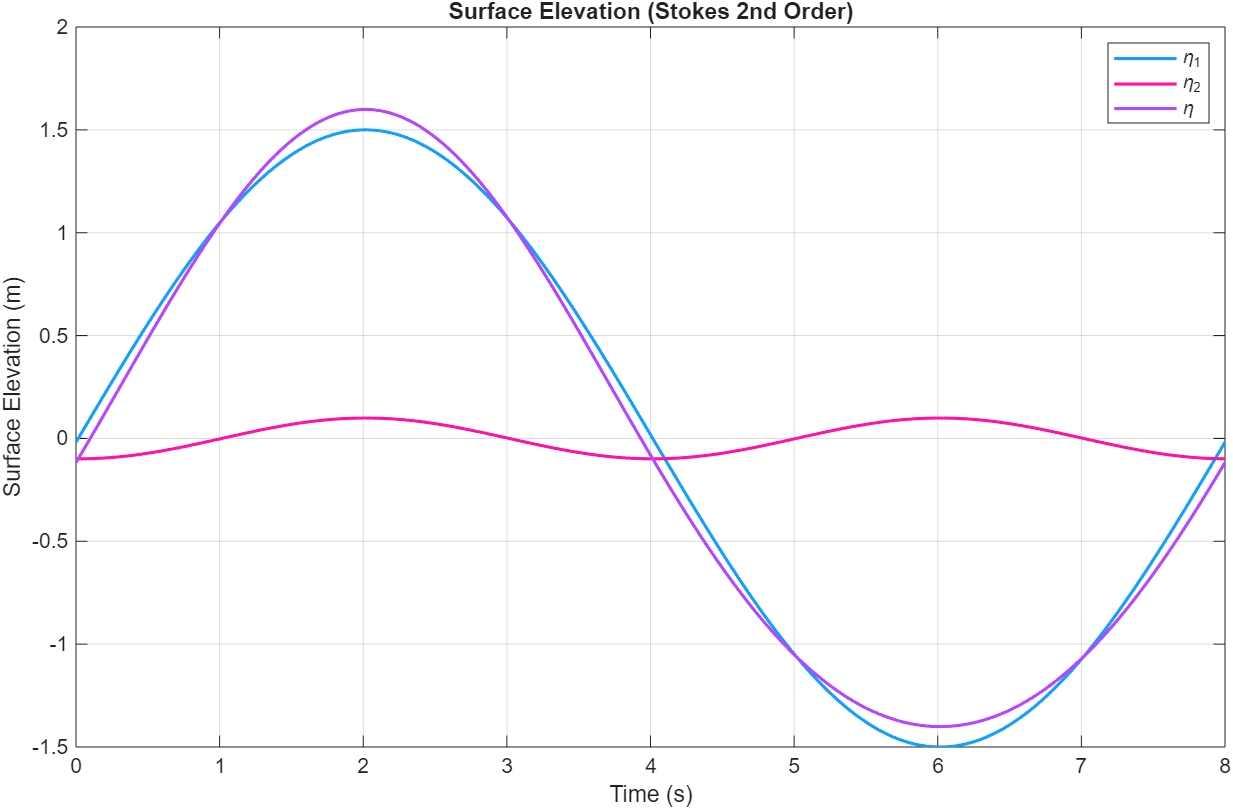
\includegraphics[width=0.6\textwidth]{CE591HW1-Q1a.png}
    \caption{\small Surface elevation plot for Stokes' second-order wave theory.}
    \label{fig:plot2a}
\end{figure}
\vspace{0.3cm}

The surface elevation plot illustrates Stokes’ second-order wave theory, combining a first-order sinusoidal wave ($\eta_1$) and a smaller second-order correction ($\eta_2$). The linear term ($\eta_1$) dominates the wave shape, while $\eta_2$ introduces asymmetry by sharpening crests and flattening troughs. At crests, $\eta_2$ adds to $\eta_1$, increasing peak height. At troughs, $\eta_2$ opposes $\eta_1$, reducing depth. The second-order term remains minor caused by the weak non-linearity. This confirms Stokes’ theory accurately models wave steepening under the given conditions.
\vspace{0.3cm}

\textbf{(b)} Make a plot of the vertical variation of horizontal (\(u\)) and vertical (\(w\)) particle velocities
\begin{figure}[H]
    \centering
    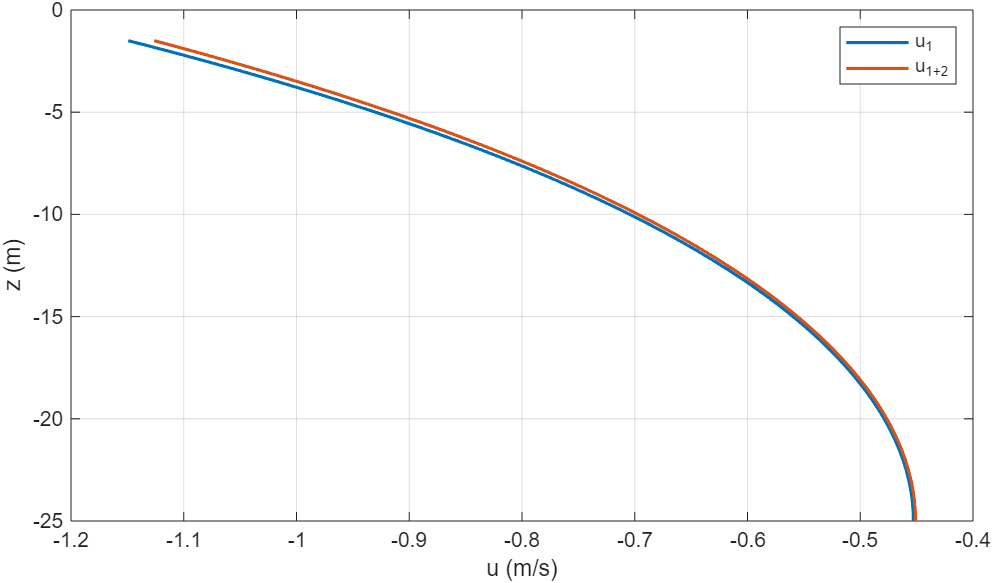
\includegraphics[width=0.8\textwidth]{CE591HW1-Q1b.png}
    \caption{\small Velocity profiles for Stokes' second-order wave theory.}
    \label{fig:plot2b}
\end{figure}
\vspace{0.3cm}

The velocity profiles illustrate the decay of horizontal (\(u\)) and vertical (\(w\)) velocities with depth. At \(t = 0\), the vertical velocity (\(w\)) peaks near the surface and diminishes to zero at the seabed, aligning with linear theory due to the cancellation of second-order terms (\(\sin(2\theta) = 0\)). The horizontal velocity (\(u\)) exhibits a slight non-zero value near the surface in Stokes' theory, exceeding the linear prediction due to second-order corrections. Both components weaken with depth, consistent with theoretical behavior. The results validate Stokes' framework in capturing depth-dependent velocity trends under the given conditions.  
\vspace{0.3cm}

\textbf{(c)} Repeat the calculations in Part (b), changing the water depth as \( h = 20 \, \text{m} \) and \( h = 30 \, \text{m} \). Compare your results with your results from Part (b).
\vspace{0.3cm}


Changing the water depth to \( h = 20 \, \text{m} \) and \( h = 30 \, \text{m} \) alters the velocity profiles:  

\begin{itemize}  
    \item {Shallower depth (\( h = 20 \, \text{m} \))}: Increased bottom influence causes the horizontal velocity to intensify near the surface due to energy concentration, while vertical velocity exhibits more rapid decrease with depth as bottom boundary effects become more dominant.\( u \). 
    \begin{figure}[H]
        \centering
        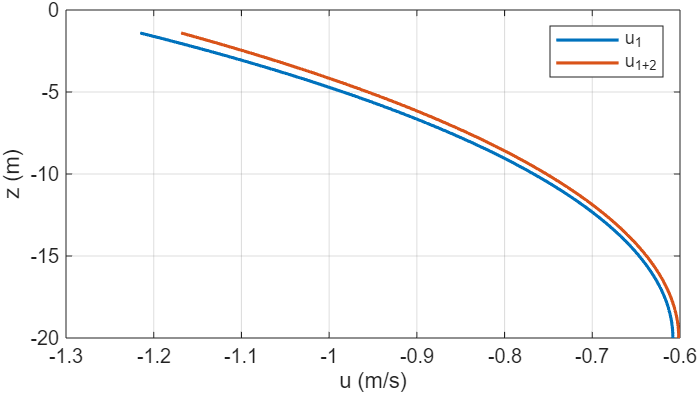
\includegraphics[width=0.8\textwidth]{CE591HW1-Q1c1.png}
        \caption{\small Velocity profiles for h = 20 m.}
        \label{fig:plot2c_1}
    \end{figure} 
    \item {Deeper depth (\( h = 30 \, \text{m} \))}: Bottom inffluence decreases with increased depth. The horizontal velocity weakens near the surface, while the vertical velocity decays more gradually with depth. 
    \begin{figure}[H]
        \centering
        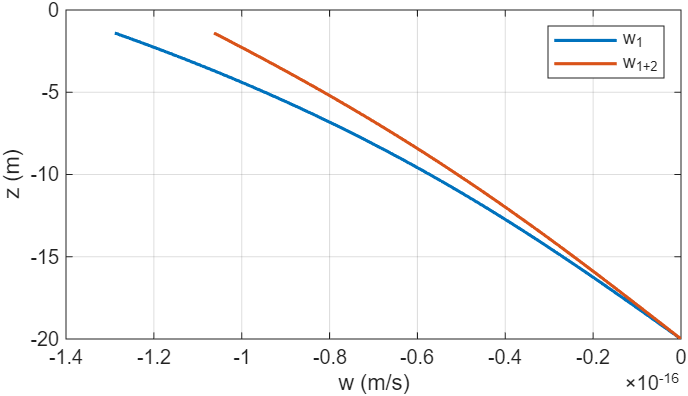
\includegraphics[width=0.8\textwidth]{CE591HW1-Q1c2.png}
        \caption{\small Velocity profiles for h = 30 m.}
        \label{fig:plot2c_2}
    \end{figure} 
\end{itemize}  
\vspace{0.5cm}

\textbf{(d)} Non-dimensional dynamic pressure can be calculated by dividing the dynamic pressure with $\rho$g$\eta$. Plot the vertical variation of the non-dimensional dynamic pressure as a function of z/h at \( h = 20 \, \text{m} \), \( h = 25 \, \text{m} \) and \( h = 30 \, \text{m} \).
\vspace{0.3cm}

\begin{figure}[H]
    \centering
    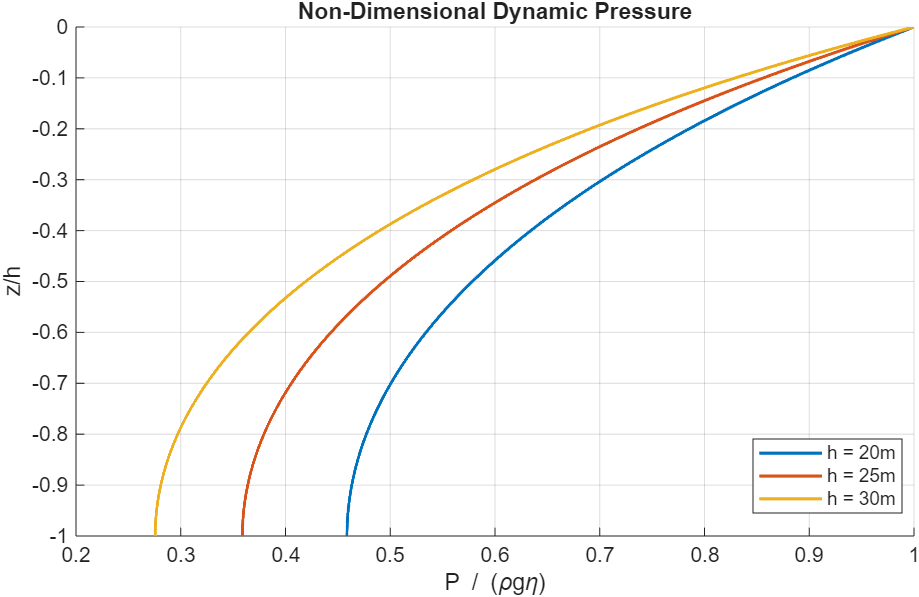
\includegraphics[width=0.8\textwidth]{CE591HW1-Q1d.png}
    \caption{\small Dynamic pressure profiles for different water depths.}
    \label{fig:plot2d}
\end{figure} 
\vspace{0.3cm}

The non-dimensional dynamic pressure profiles show how the pressure decreases with depth for different water depths. The pressure gradually decreases from the surface to the seabed. In shallower water, the pressure stays stronger with depth. This is caused by the wave energy being squeezed into a smaller volume of water, making the push from the wave more noticable near the seabed. In deeper water, the pressure weakens faster with depth, as the wave energy spreads out.
\vspace{0.5cm}

\textbf{Question 3:} Write a program that calculates the water surface elevation of a solitary wave for a given solitary wave height H and water depth h. Plot the water surface elevation for H = 0.074 m and h = 30 cm. Compare your theoretical calculation and experimental measurements. Discuss potential discrepancies.
\vspace{0.3cm}

\begin{figure}[H]
    \centering
    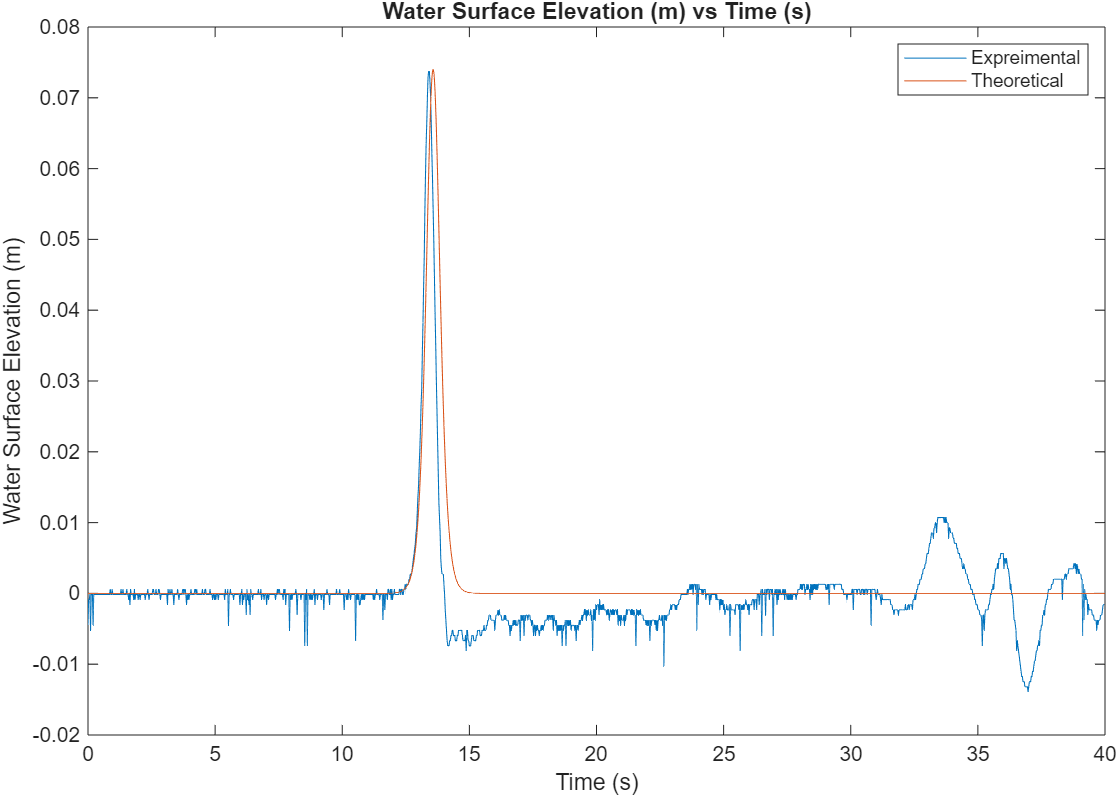
\includegraphics[width=0.8\textwidth]{CE591HW1-Q3.png}
    \caption{\small Surface elevation of a solitary wave.}
    \label{fig:plot3}
\end{figure} 
\vspace{0.3cm}

The comparison between theoretical and experimental solitary wave profiles shows a good match, with some expected discrepancies. The theoretical model assumes ideal conditions, while experimental data may be influenced by factors like wave reflection, bottom friction, and measurement errors. The solitary wave's shape is quite similar, but the amplitude and width shows slight differences due to these real-world effects. The experimental data also shows some oscillations, likely caused by wave interactions or reflections. Overall, the theoretical model provides a solid foundation for solitary waves, but real-world conditions can introduce variations that need to be considered in practical applications.
\vspace{0.5cm}

\textbf{Question 4:} Write a program utilizing cnoidal wave theory summarized in your lecture notes for a given wave height H, wave period T and water depth h. Plot the water surface elevations for at least three selected waves on the same figure for two wave periods. Describe the procedure you have used and discuss your results.
\vspace{0.3cm}

\textbf{Procedure:} The MATLAB program calculates the water surface elevation of cnoidal waves using the following steps:

1. The wave height \(H\), wave period \(T\), and water depth \(h\) were chosen to be within the applicable area for cnoidal waves.

2. Within the function, there are two nested loops. The outer loop is for calculating the \(Ur\) value for the given wave parameters using \(L_c\) and the inner loop is for calculating the \(m\) value for each value of \(Ur\). With this m value, a new \(Ur\) is calculated. After these values converge, the surface elevation ($\eta$) is calculated using the cnoidal wave formula.

3. The program then plots the surface elevation, showing how the wave shape changes with time.
\vspace{0.3cm}

The inner loop calculating m is based on the following equations:

\[A = 1 \]
\[ L_c = T \cdot \sqrt{\frac{g}{h}} \cdot \sqrt{1 + \frac{H}{h} \cdot A[m]} \cdot h \]
\[U_r = H \cdot \frac{L_c^2}{h^3} \]     
\[m_{1,0} = \exp\left(\frac{a_0 - \sqrt{3 \cdot \frac{U_r}{16}}}{b_0}\right)\]
\[K[m_1] = \left(a_0 + a_1 m_1 + a_2 m_1^2\right) - \left(b_0 + b_1 m_1 + b_2 m_1^2\right) \ln(m_1)\]
\[f(m_1) = 1 - m_1 - \frac{3}{16} \cdot \frac{U_r}{K^2[m_1]} = 0\]
\[m_{1,i+1} = m_{1,i} - \frac{f(m_{1,i})}{f'(m_{1,i})}\]
\[m = 1 - m_1\]
\vspace{0.3cm}

The outer loop calculating the \(Ur\) uses the formula for \(L_c\) seen above. With the changing \(m_1\) value, the new \(L_c\) is calculated by iterating \(A[m]\) using the following equations:

\[E[m_1] = \left(1 + e_1 m_1 + e_2 m_1^2\right) - \left(f_1 m_1 + f_2 m_1^2\right) \ln(m_1)\]
\[A[m] = \frac{2}{m} - 1 - \frac{3}{m} \frac{E[m_1]}{K[m_1]}\]
\vspace{0.3cm}

Then, the program calculates the surface elevation using the cnoidal wave formula:

\[\eta = H \cdot \left(B + \text{cn}^2\left(K_c \cdot (x - c_c \cdot t), m\right)\right)\]

\begin{figure}[H]
    \centering
    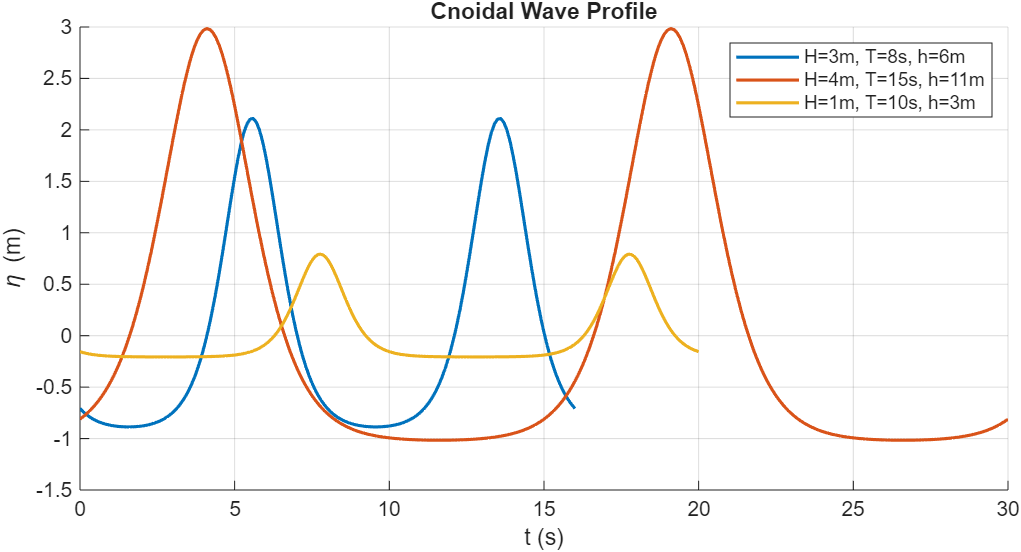
\includegraphics[width=0.8\textwidth]{CE591HW1-Q4.png}
    \caption{\small Cnoidal wave surface elevation.}
    \label{fig:plot4}
\end{figure} 
\vspace{0.3cm}

\textbf{Question 5:} In this question, you will generate a computational mesh using blockMesh utility of OpenFOAM. A wave will be generated using first-order wave theory in this flume. Generate a 2D computational mesh based on the information given.
\vspace{0.3cm}

The mesh is generated with 1 m length in z direction, 25 m length in x direction and 0.1 m height in y direction. Using these coordinates, the vertices of the block is formed in the blockMeshDict file. It is then divided into 2500 cells in x direction, 1 cell in y direction and 280 cells in z direction. To obtain the cell count for the z direction, the first cell size of $7.5 \cdot 10^{-4}$ m and last cell size of 0.01 m are used. The last cell size is selected to keep the aspect ratio equal to 1 at the free-surface. The grading on the z-direction is calculated to be 13.333 based on the first and last cell sizes and the total length.

\begin{figure}[H]
    \centering
    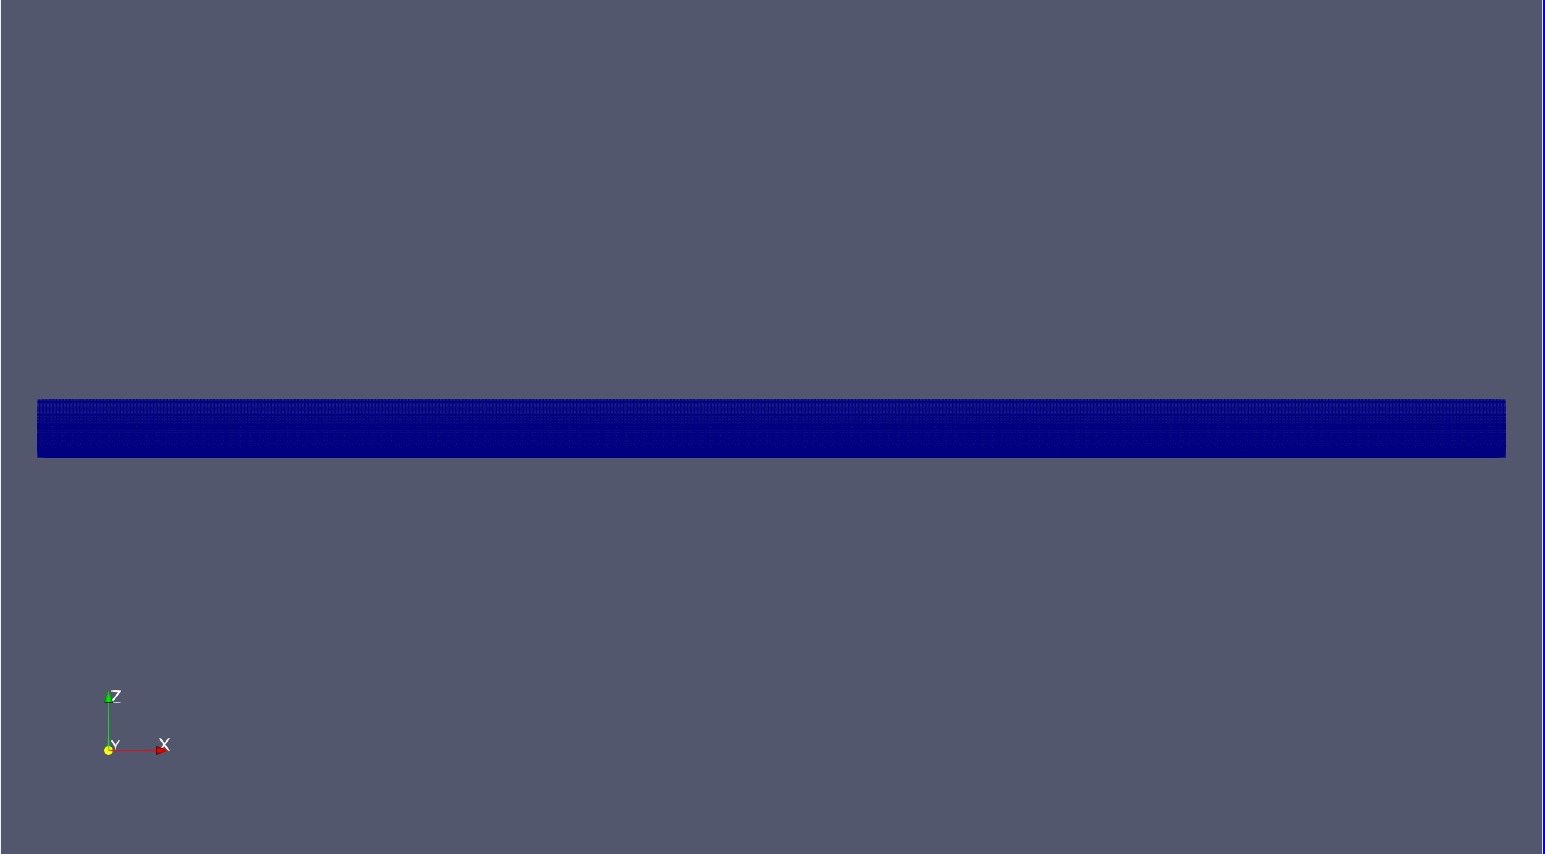
\includegraphics[width=0.6\textwidth]{mesh1.jpg}
    \caption{\small 2D computational mesh generated using blockMesh utility of OpenFOAM.}
    \label{fig:mesh1}
\end{figure} 
\vspace{0.3cm}
\begin{figure}[H]
    \centering
    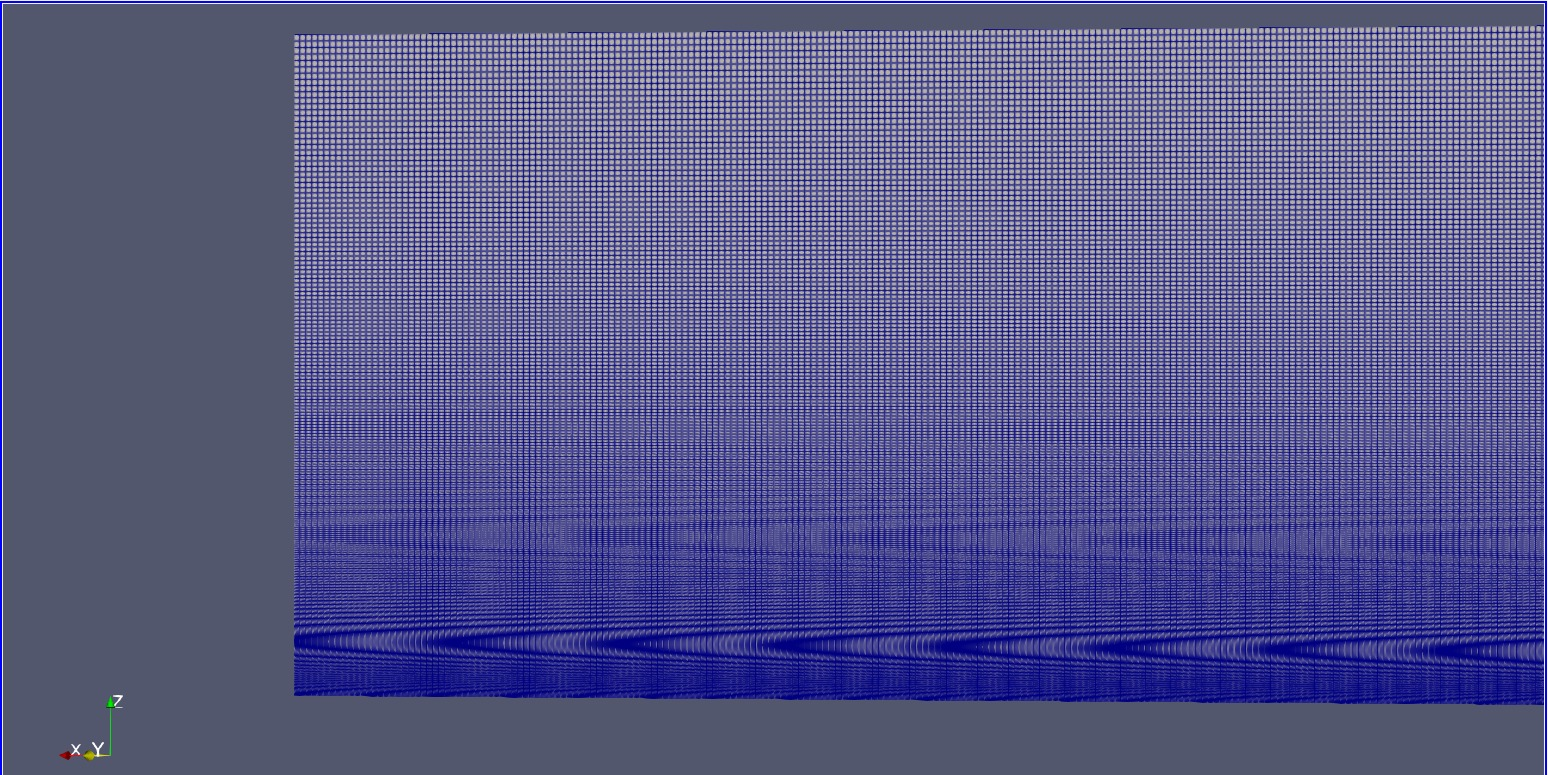
\includegraphics[width=0.6\textwidth]{mesh2.jpg}
    \caption{\small 2D computational mesh generated using blockMesh utility of OpenFOAM.}
    \label{fig:mesh2}
\end{figure} 
\vspace{0.3cm}
\begin{figure}[H]
    \centering
    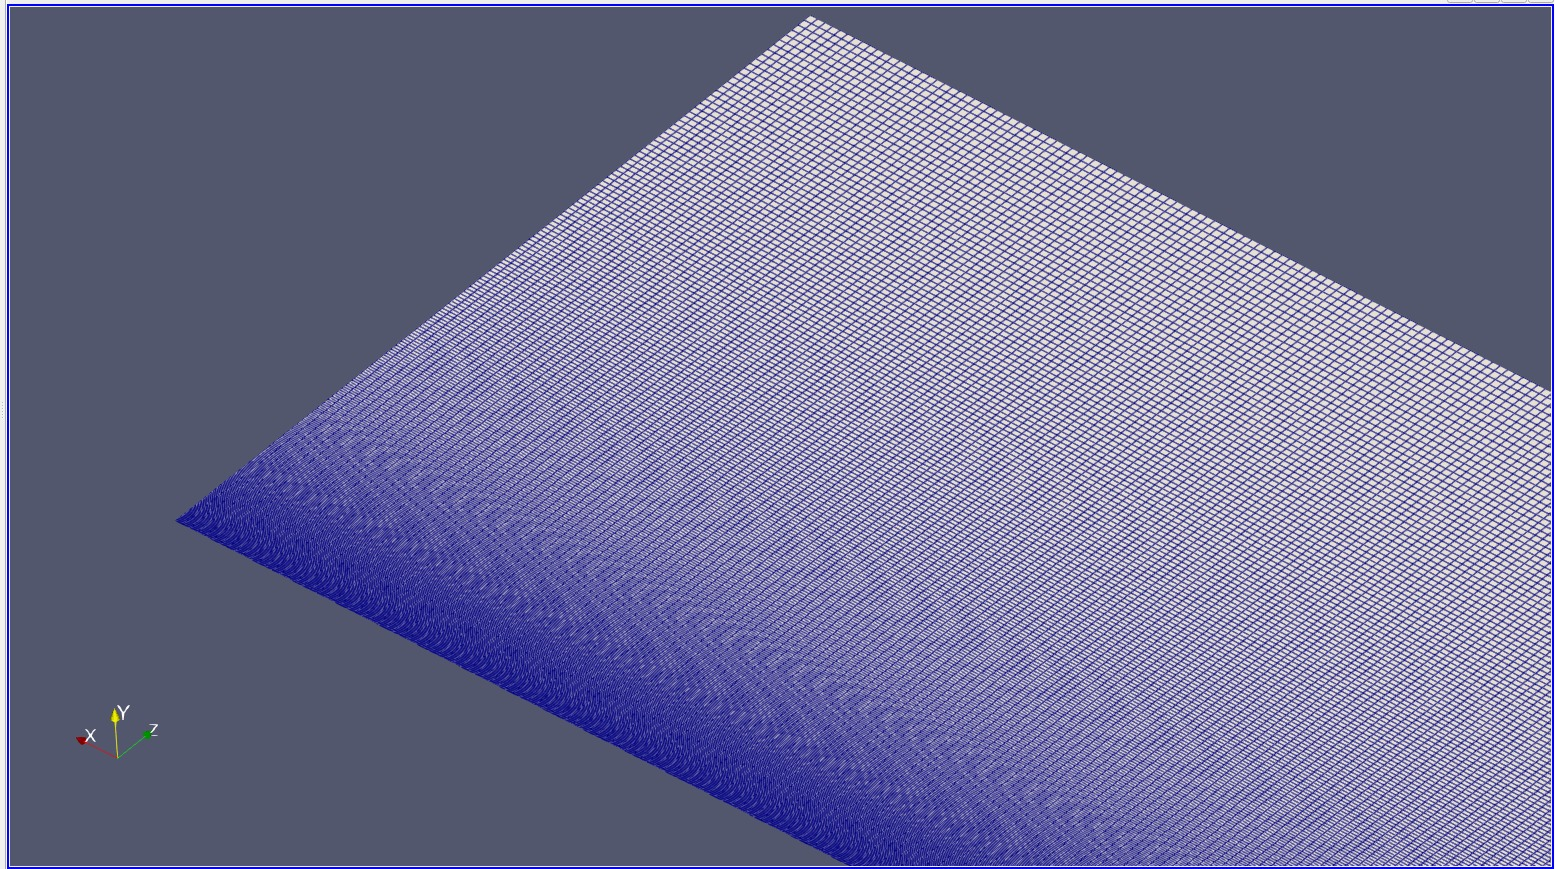
\includegraphics[width=0.6\textwidth]{mesh3.jpg}
    \caption{\small 2D computational mesh generated using blockMesh utility of OpenFOAM.}
    \label{fig:mesh3}
\end{figure} 
\vspace{0.3cm}

The total number of cells in the mesh is \textbf{700,000}, the maximum cell area is \textbf{$7.487 \cdot 10^{-6}$m}, the minimum cell area is \textbf{0.001m}, and the maximum aspect ratio is \textbf{10}, as obtained from the checkMesh function.

\end{document}